\section{Data stretch profiles}\label{sec:data_stretch_profiles}

Friction vs. stretch profiles for the kirigami data set. The mean value is taken across the three normal forces. The data points have been interpolated with a cubic spline interpolation in order to approximate the full continous curve mainly for visual purposes. 


% Honeycomb
\begin{figure}[H]
    \centering
    \begin{subfigure}[b]{0.49\textwidth}
        \centering
        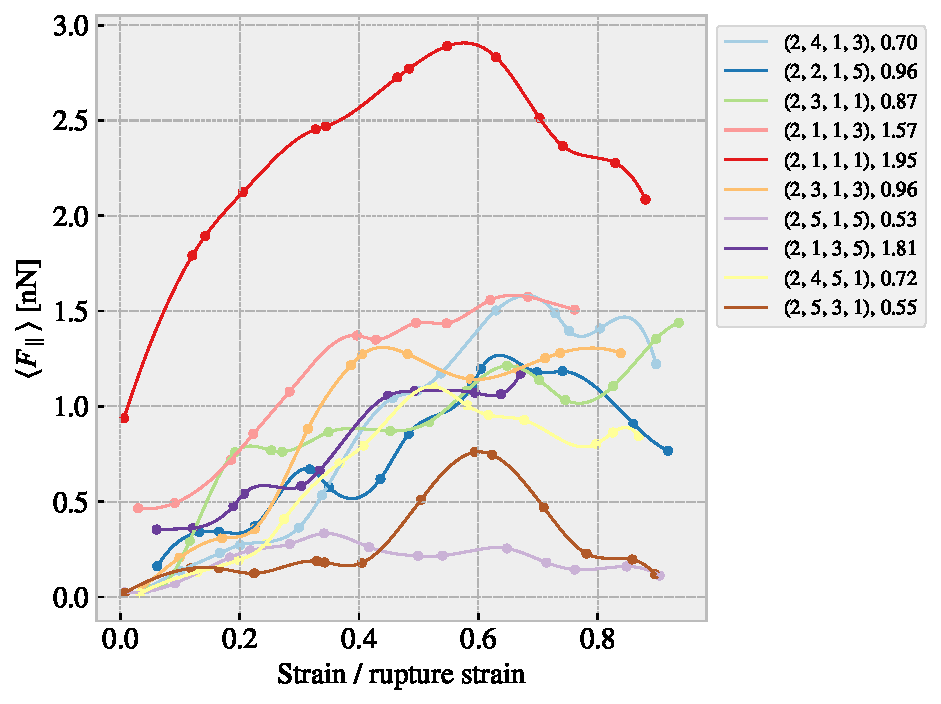
\includegraphics[width=\textwidth]{figures/stretch_profiles/honeycomb/SP_0_honeycomb.pdf}
        \caption{}
        \label{fig:}
    \end{subfigure}
    \hfill
    \begin{subfigure}[b]{0.49\textwidth}
        \centering
        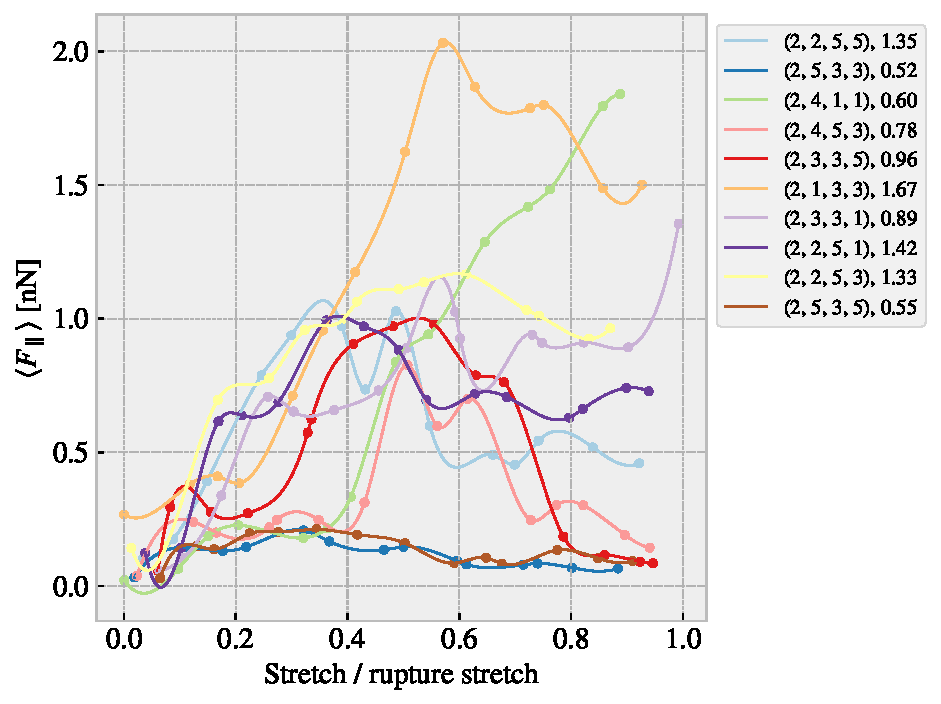
\includegraphics[width=\textwidth]{figures/stretch_profiles/honeycomb/SP_1_honeycomb.pdf}
        \caption{}
        \label{fig:}
    \end{subfigure}
    \hfill
    \begin{subfigure}[b]{0.49\textwidth}
        \centering
        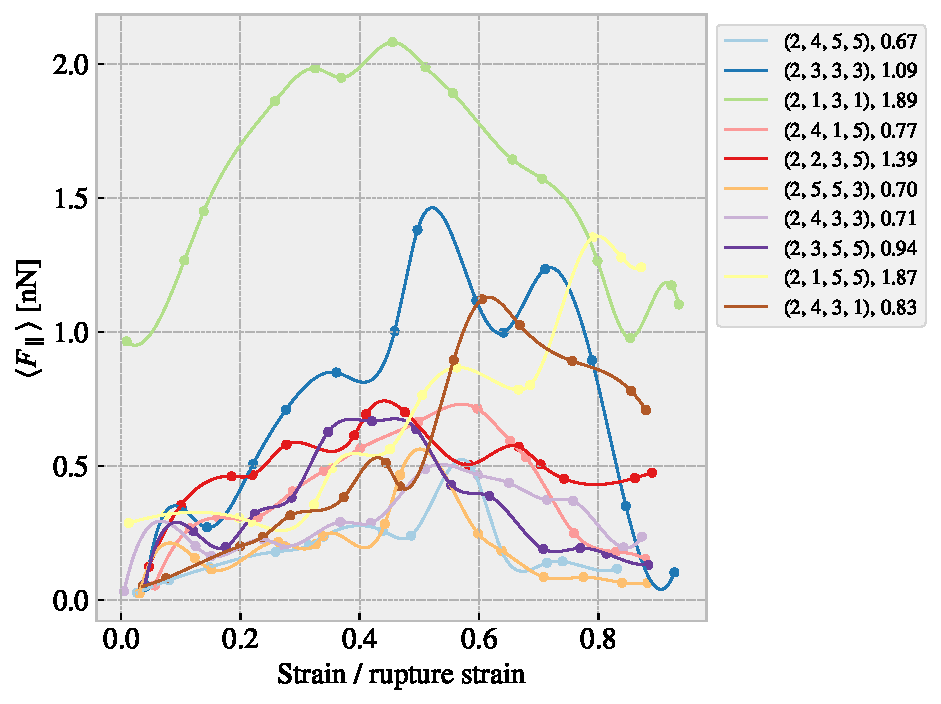
\includegraphics[width=\textwidth]{figures/stretch_profiles/honeycomb/SP_2_honeycomb.pdf}
        \caption{}
        \label{fig:}
    \end{subfigure}
    \hfill
    \begin{subfigure}[b]{0.49\textwidth}
        \centering
        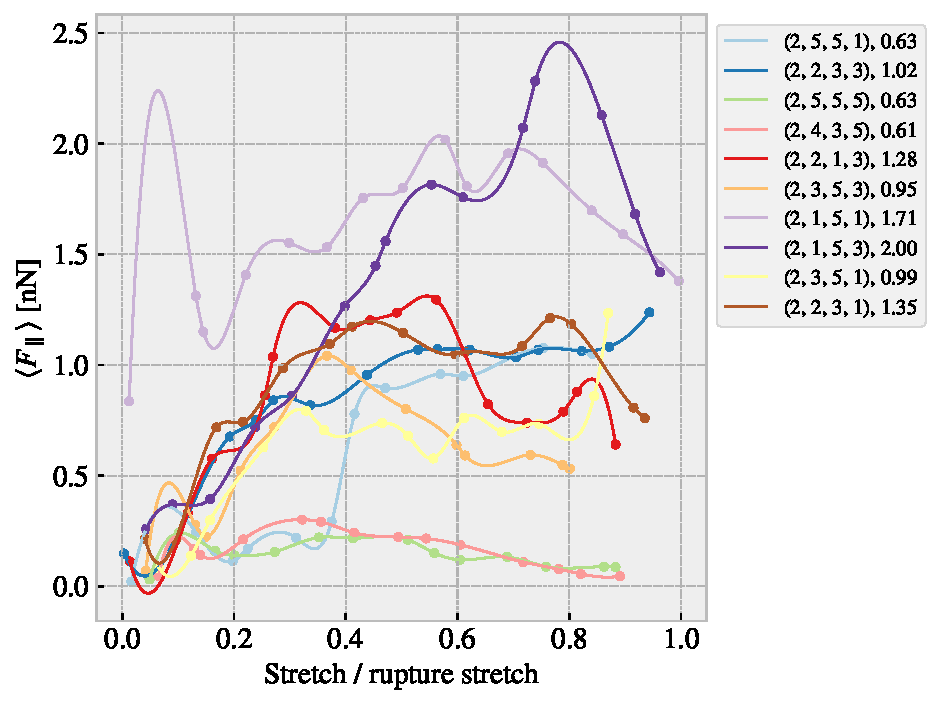
\includegraphics[width=\textwidth]{figures/stretch_profiles/honeycomb/SP_3_honeycomb.pdf}
        \caption{}
        \label{fig:}
    \end{subfigure}
    \hfill
    \caption{Honeycomb.}
    \label{fig:}
\end{figure}


%Popup
\begin{figure}[H]
    \centering
    \begin{subfigure}[b]{0.49\textwidth}
        \centering
        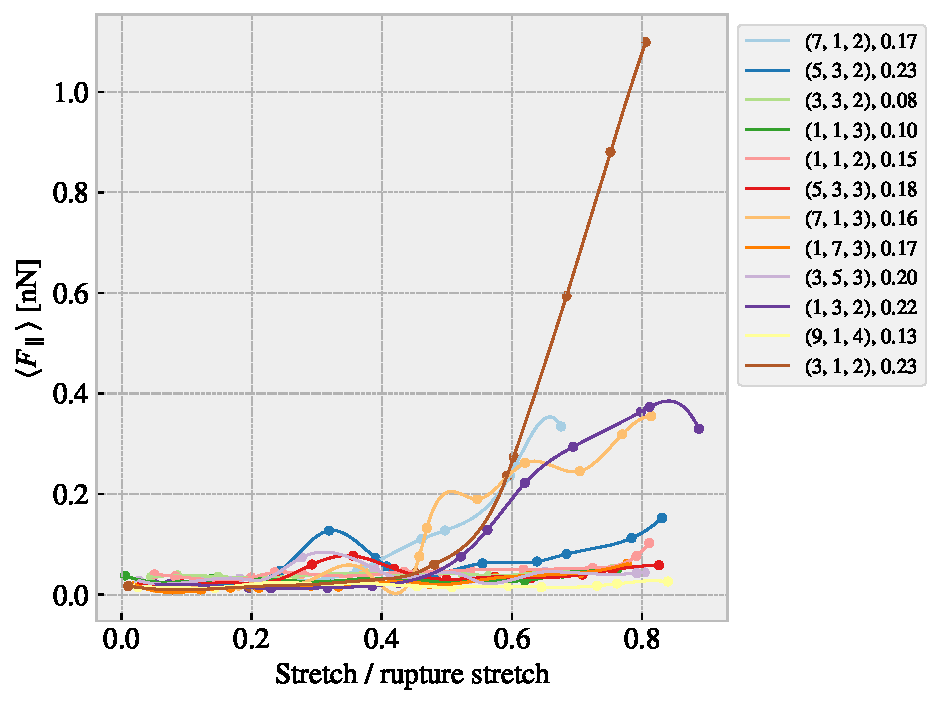
\includegraphics[width=\textwidth]{figures/stretch_profiles/popup/SP_0_popup.pdf}
        \caption{}
        \label{fig:}
    \end{subfigure}
    \hfill
    \begin{subfigure}[b]{0.49\textwidth}
        \centering
        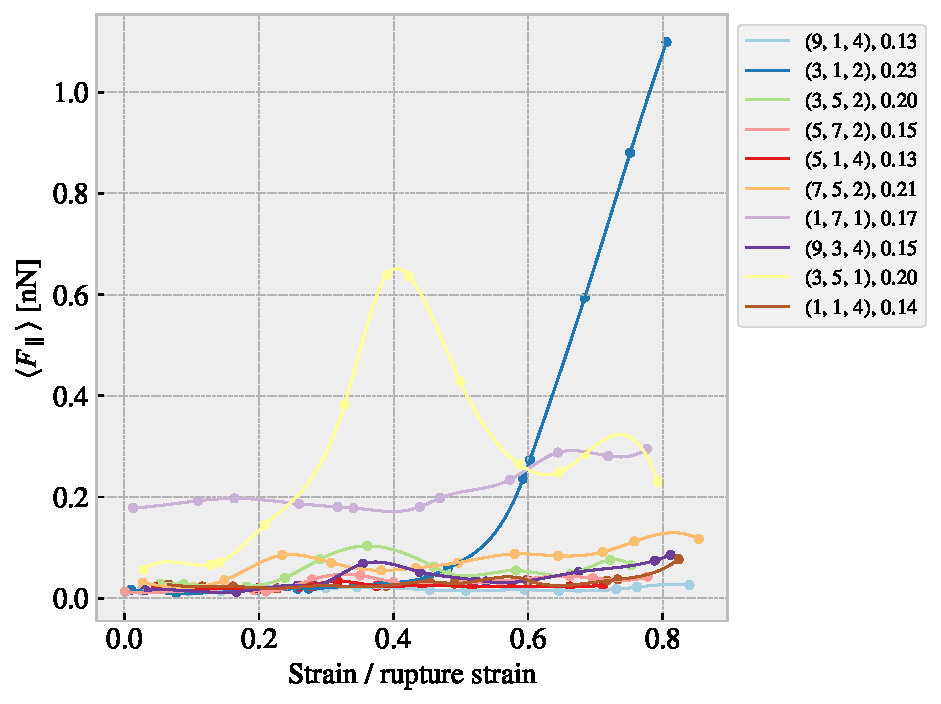
\includegraphics[width=\textwidth]{figures/stretch_profiles/popup/SP_1_popup.pdf}
        \caption{}
        \label{fig:}
    \end{subfigure}
    \hfill
    \begin{subfigure}[b]{0.49\textwidth}
        \centering
        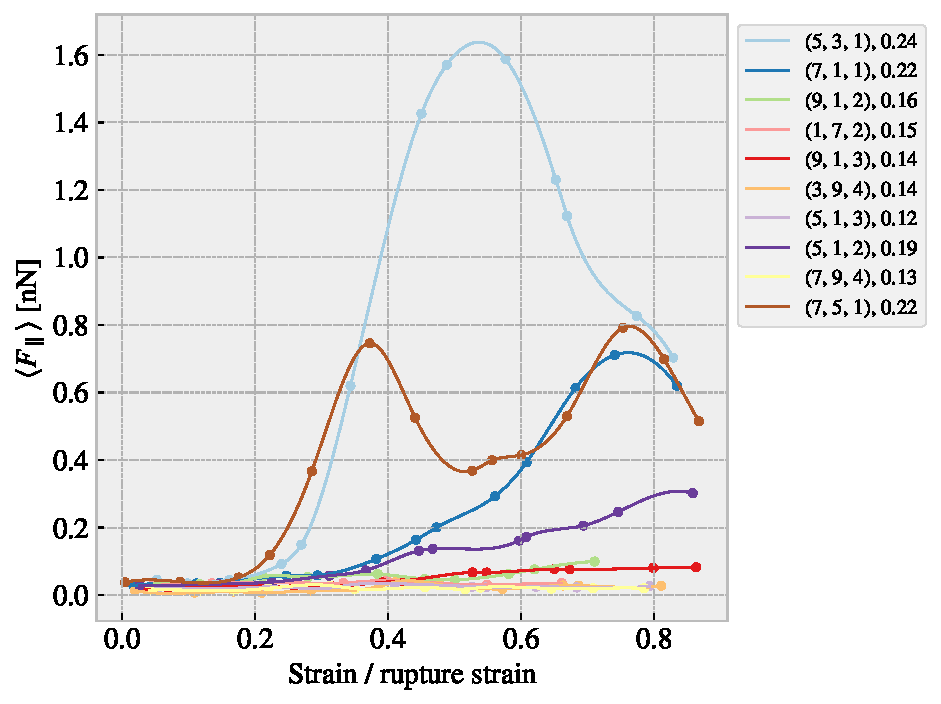
\includegraphics[width=\textwidth]{figures/stretch_profiles/popup/SP_2_popup.pdf}
        \caption{}
        \label{fig:}
    \end{subfigure}
    \hfill
    \begin{subfigure}[b]{0.49\textwidth}
        \centering
        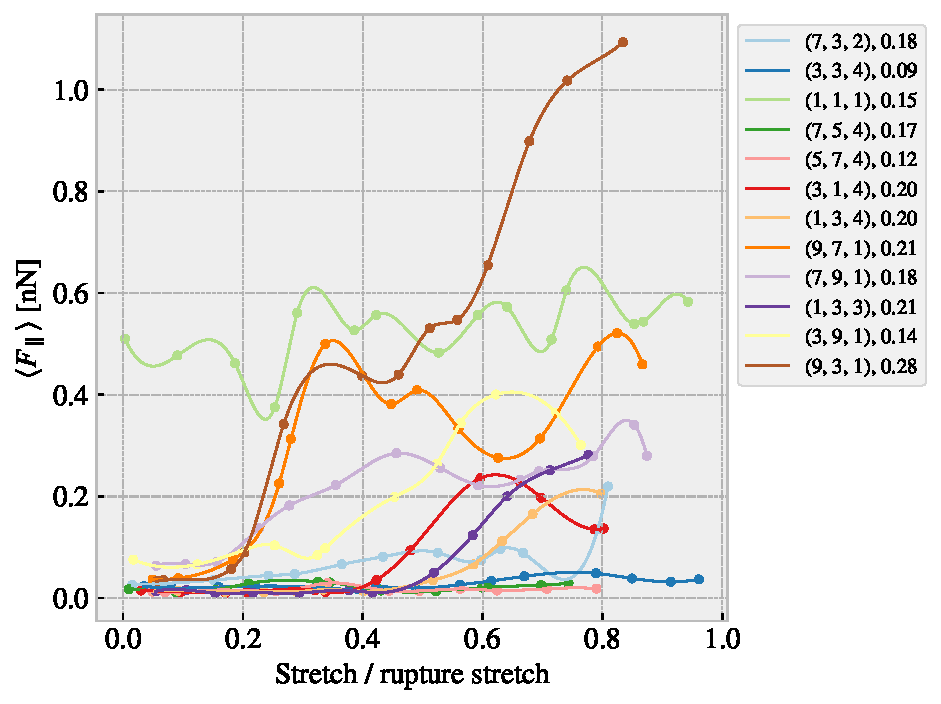
\includegraphics[width=\textwidth]{figures/stretch_profiles/popup/SP_3_popup.pdf}
        \caption{}
        \label{fig:}
    \end{subfigure}
    \hfill
    \begin{subfigure}[b]{0.49\textwidth}
        \centering
        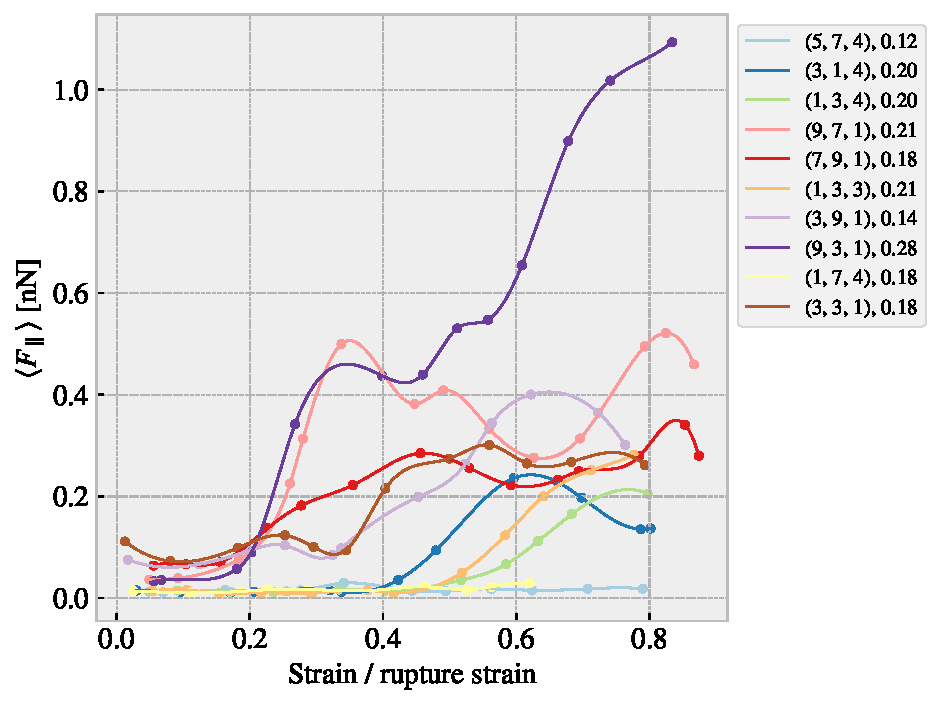
\includegraphics[width=\textwidth]{figures/stretch_profiles/popup/SP_4_popup.pdf}
        \caption{}
        \label{fig:}
    \end{subfigure}
    \hfill
    \begin{subfigure}[b]{0.49\textwidth}
        \centering
        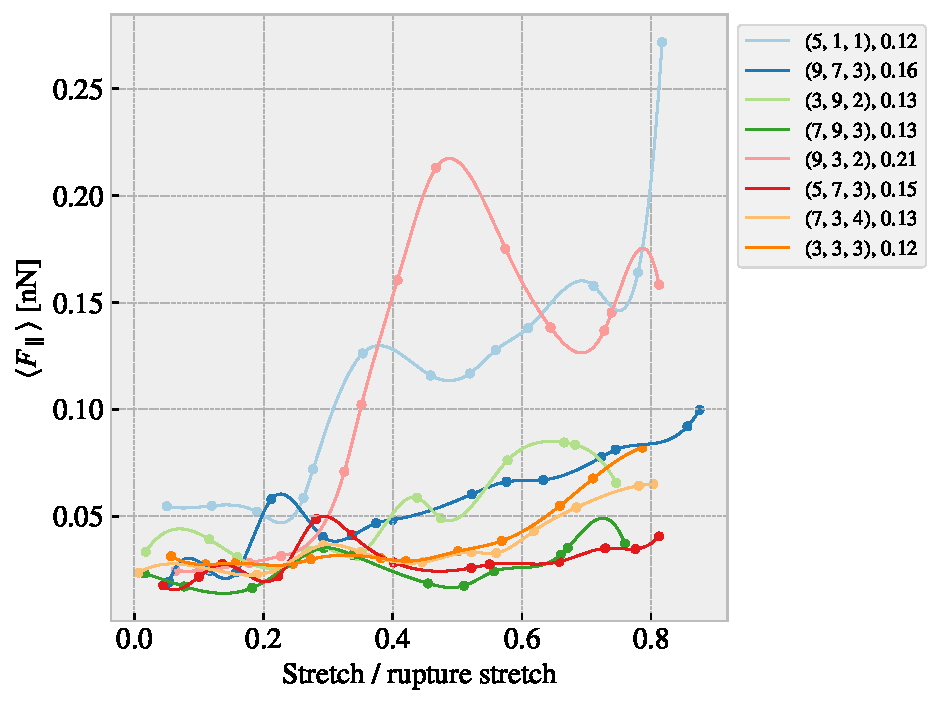
\includegraphics[width=\textwidth]{figures/stretch_profiles/popup/SP_5_popup.pdf}
        \caption{}
        \label{fig:}
    \end{subfigure}
    \hfill
    \caption{Tetrahedron.}
    \label{fig:}
\end{figure}



%RW
\begin{figure}[H]
    \centering
    \begin{subfigure}[b]{0.49\textwidth}
        \centering
        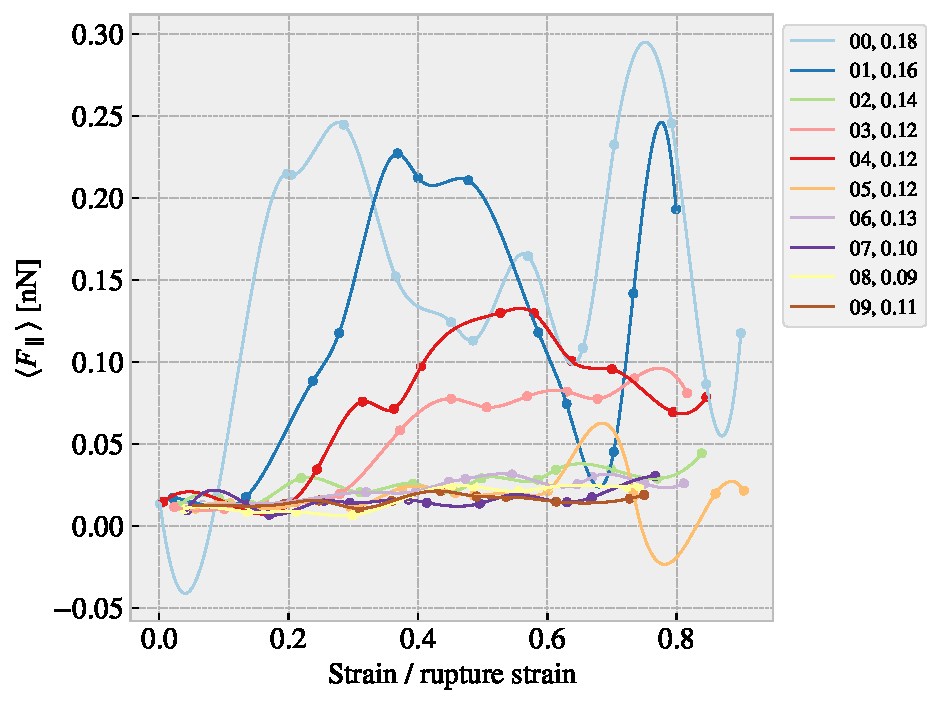
\includegraphics[width=\textwidth]{figures/stretch_profiles/RW/SP_0_RW.pdf}
        \caption{}
        \label{fig:}
    \end{subfigure}
    \hfill
    \begin{subfigure}[b]{0.49\textwidth}
        \centering
        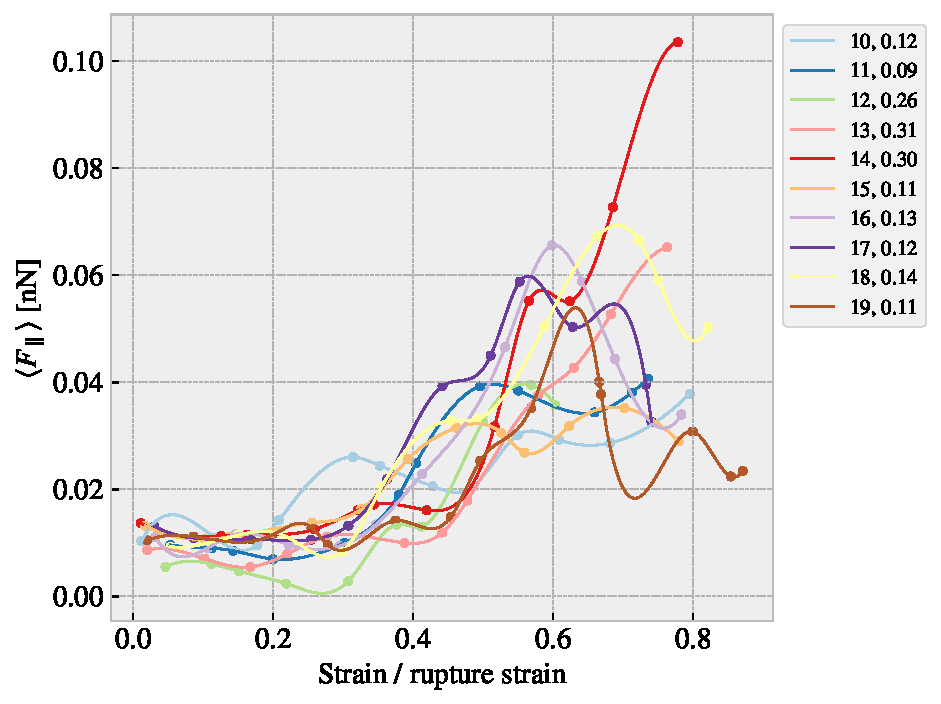
\includegraphics[width=\textwidth]{figures/stretch_profiles/RW/SP_1_RW.pdf}
        \caption{}
        \label{fig:}
    \end{subfigure}
    \hfill
    \begin{subfigure}[b]{0.49\textwidth}
        \centering
        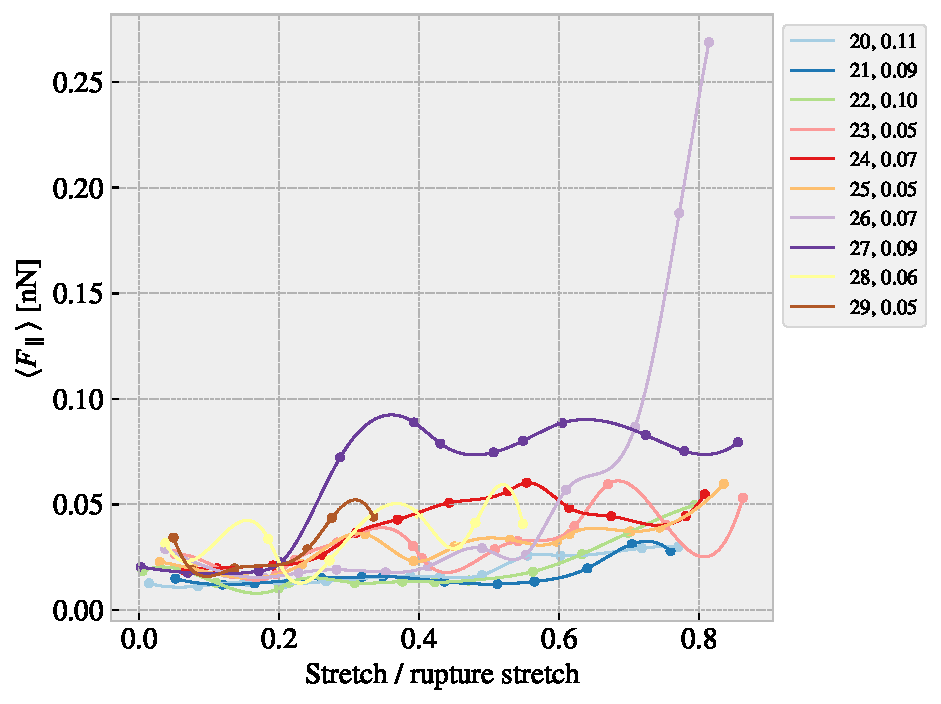
\includegraphics[width=\textwidth]{figures/stretch_profiles/RW/SP_2_RW.pdf}
        \caption{}
        \label{fig:}
    \end{subfigure}
    \hfill
    \begin{subfigure}[b]{0.49\textwidth}
        \centering
        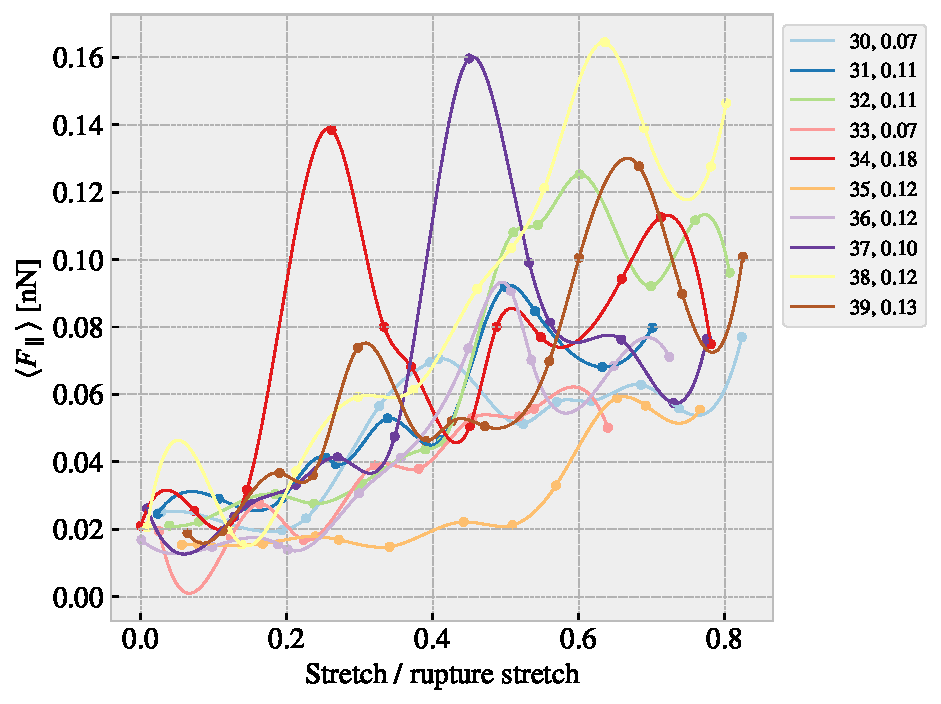
\includegraphics[width=\textwidth]{figures/stretch_profiles/RW/SP_3_RW.pdf}
        \caption{}
        \label{fig:}
    \end{subfigure}
    \hfill
    \begin{subfigure}[b]{0.49\textwidth}
        \centering
        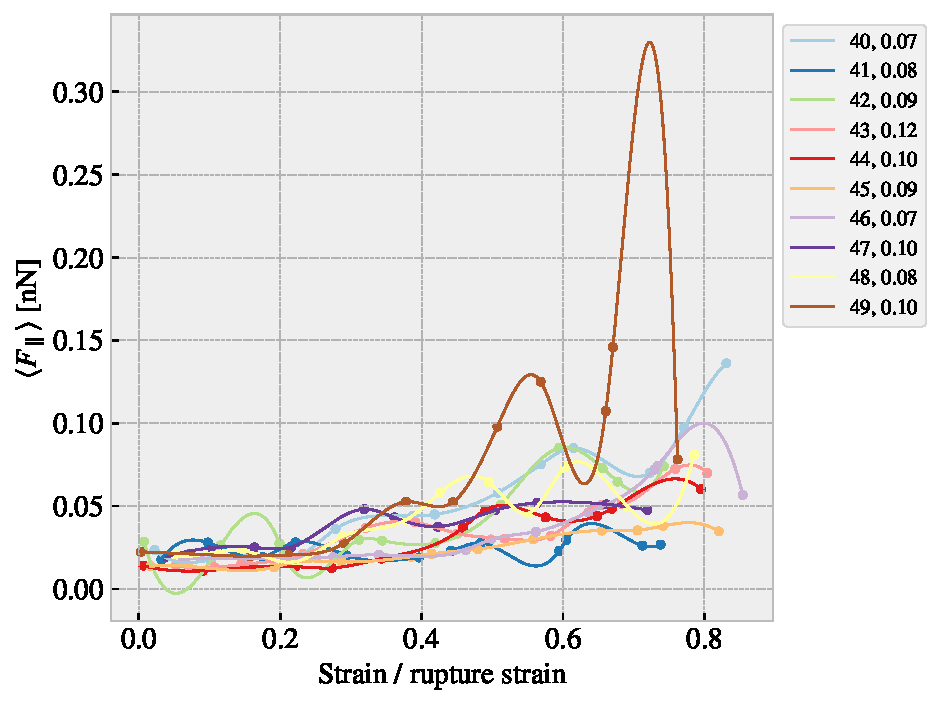
\includegraphics[width=\textwidth]{figures/stretch_profiles/RW/SP_4_RW.pdf}
        \caption{}
        \label{fig:}
    \end{subfigure}
    \hfill
    \begin{subfigure}[b]{0.49\textwidth}
        \centering
        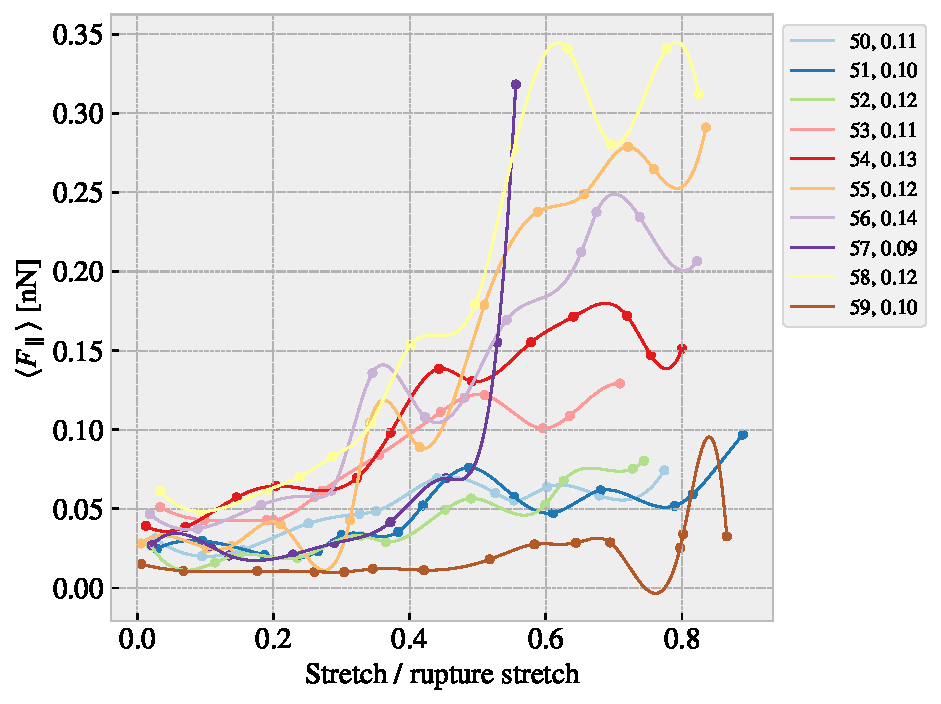
\includegraphics[width=\textwidth]{figures/stretch_profiles/RW/SP_5_RW.pdf}
        \caption{}
        \label{fig:}
    \end{subfigure}
    \hfill
    \caption{Random walk.}
    \label{fig:}
\end{figure}


\begin{figure}[H]
    \centering
    \begin{subfigure}[b]{0.49\textwidth}
        \centering
        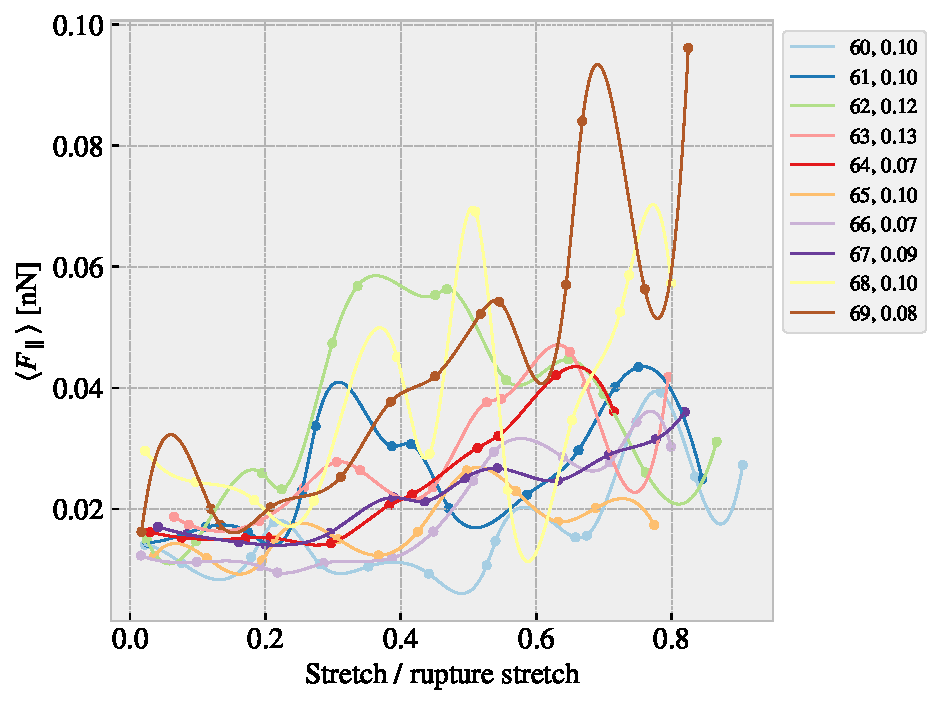
\includegraphics[width=\textwidth]{figures/stretch_profiles/RW/SP_6_RW.pdf}
        \caption{}
        \label{fig:}
    \end{subfigure}
    \hfill
    \begin{subfigure}[b]{0.49\textwidth}
        \centering
        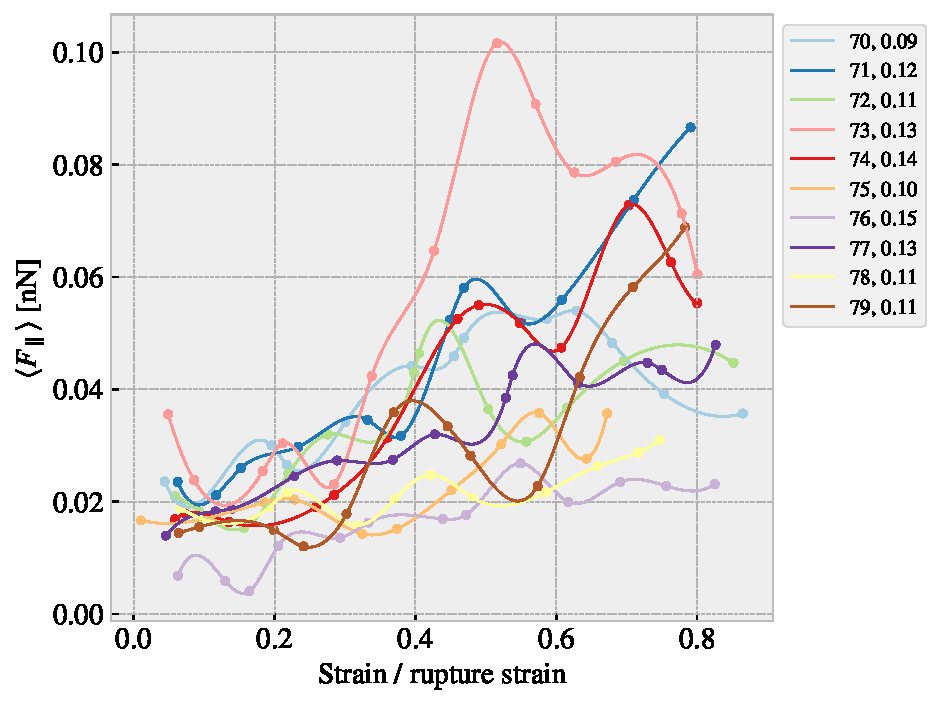
\includegraphics[width=\textwidth]{figures/stretch_profiles/RW/SP_7_RW.pdf}
        \caption{}
        \label{fig:}
    \end{subfigure}
    \hfill
    \begin{subfigure}[b]{0.49\textwidth}
        \centering
        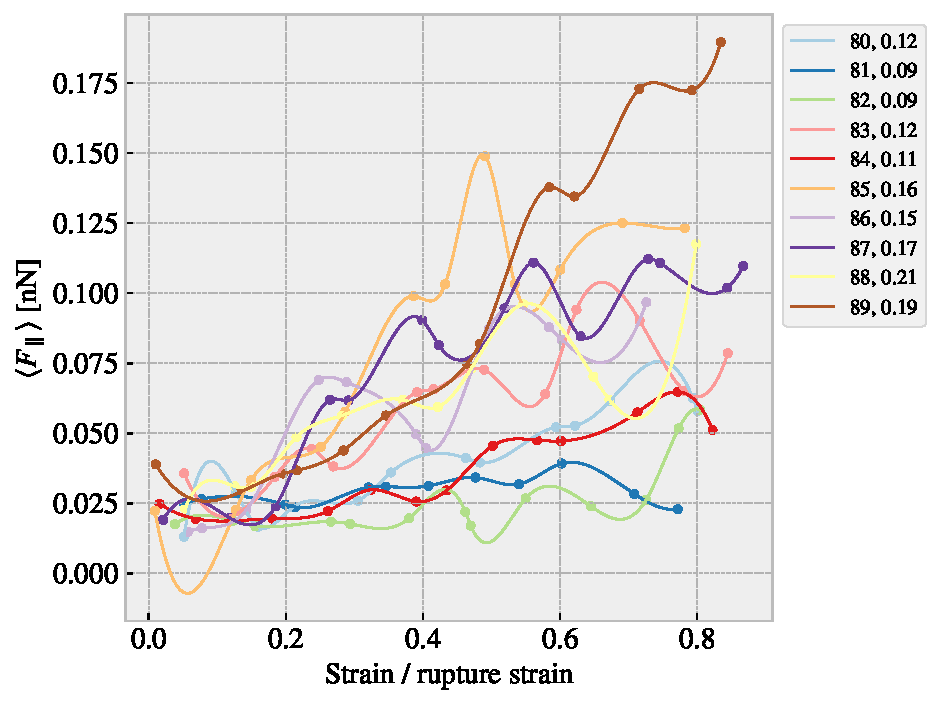
\includegraphics[width=\textwidth]{figures/stretch_profiles/RW/SP_8_RW.pdf}
        \caption{}
        \label{fig:}
    \end{subfigure}
    \hfill
    \begin{subfigure}[b]{0.49\textwidth}
        \centering
        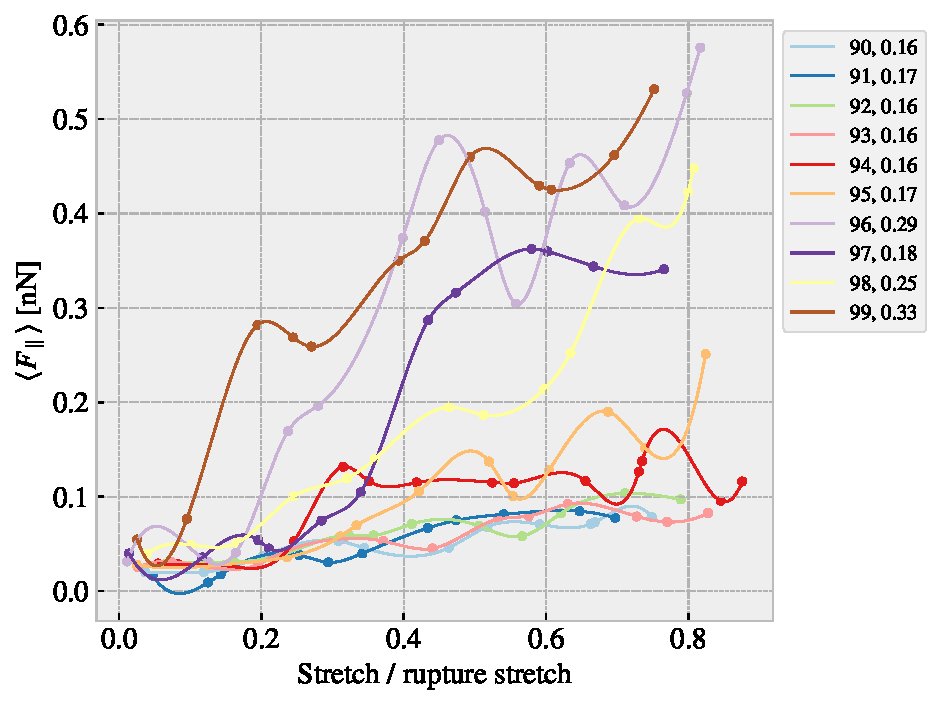
\includegraphics[width=\textwidth]{figures/stretch_profiles/RW/SP_9_RW.pdf}
        \caption{}
        \label{fig:}
    \end{subfigure}
    \hfill
    \caption{Random walk.}
    \label{fig:}
\end{figure}
